\documentclass{beamer}
\usepackage{amsmath}
\usetheme{Singapore}
\title{Leverage the power of the First Order... Logic: Introduction to TLA+}
\author{Thomas Bracher}
\date{\today}
\setbeamertemplate{navigation symbols}{}

\begin{document}
\maketitle
\begin{frame}
  \frametitle{Different Paradigms, same goal}
  \begin{itemize}
    \item C -- procedural
    \item Java -- object oriented
    \item Haskell -- functional
    \item Built for code execution
  \end{itemize}
\end{frame}

\begin{frame}
  \frametitle{Enters TLA+}
  \begin{columns}
    \begin{column}{0.5\textwidth}
      Specification language by Leslie Lamport
    \end{column}
    \begin{column}{0.5\textwidth}
      \begin{center}
        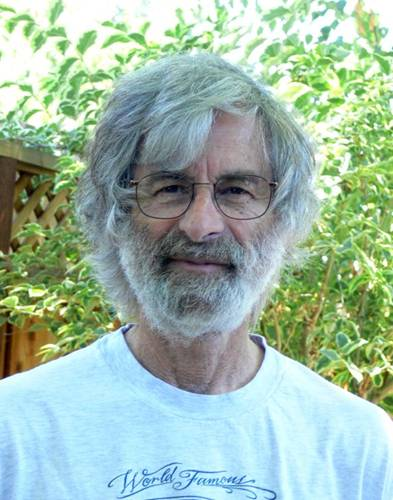
\includegraphics[width=0.5\textwidth]{tla-introduction/leslie}
      \end{center}
    \end{column}
  \end{columns}
\end{frame}

\begin{frame}
  \frametitle{TLA+: Temporal Logic Action}
  \begin{itemize}
    \item Temporal = intuitive time
    \item Logical = first order logic
    \item Action = why not?
  \end{itemize}
\end{frame}

\begin{frame}
  \frametitle{Reservation Train Kata}
  \begin{figure}
    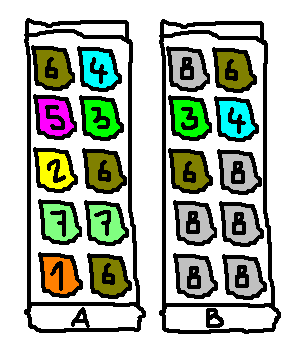
\includegraphics[scale=0.7]{tla-introduction/other-configuration}
  \end{figure}
\end{frame}

\begin{frame}
  \frametitle{The Rules}
  \begin{figure}
    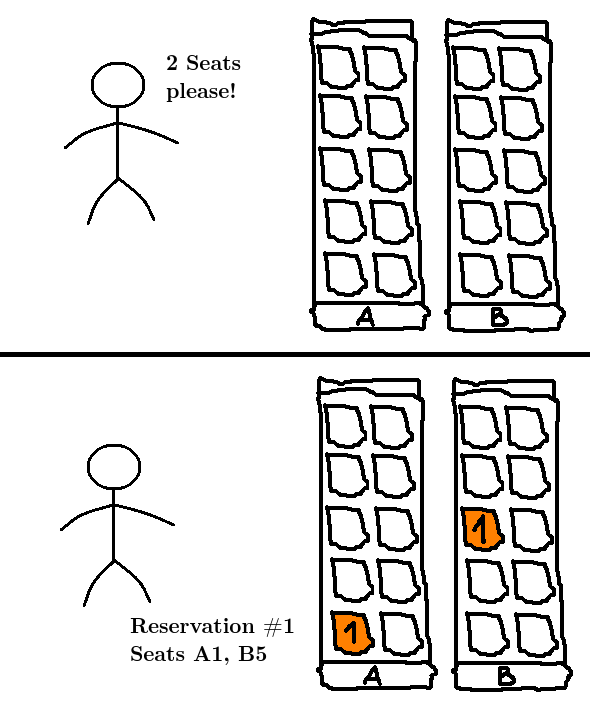
\includegraphics[scale=0.4]{tla-introduction/client-reserving}
  \end{figure}
\end{frame}

\begin{frame}
  \frametitle{The Rules}
  \begin{columns}
    \begin{column}{0.5\textwidth}
      Max 70\% occupation
    \end{column}
    \begin{column}{0.5\textwidth}
      \begin{center}
        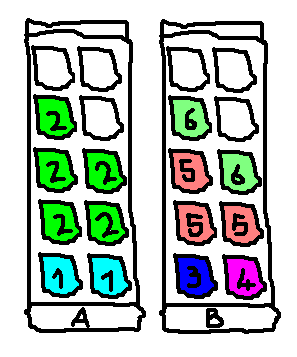
\includegraphics[width=0.5\textwidth]{tla-introduction/compliant-train}
      \end{center}
    \end{column}
  \end{columns}
\end{frame}

\begin{frame}
  \frametitle{Enters the First Order...}
  \begin{center}
    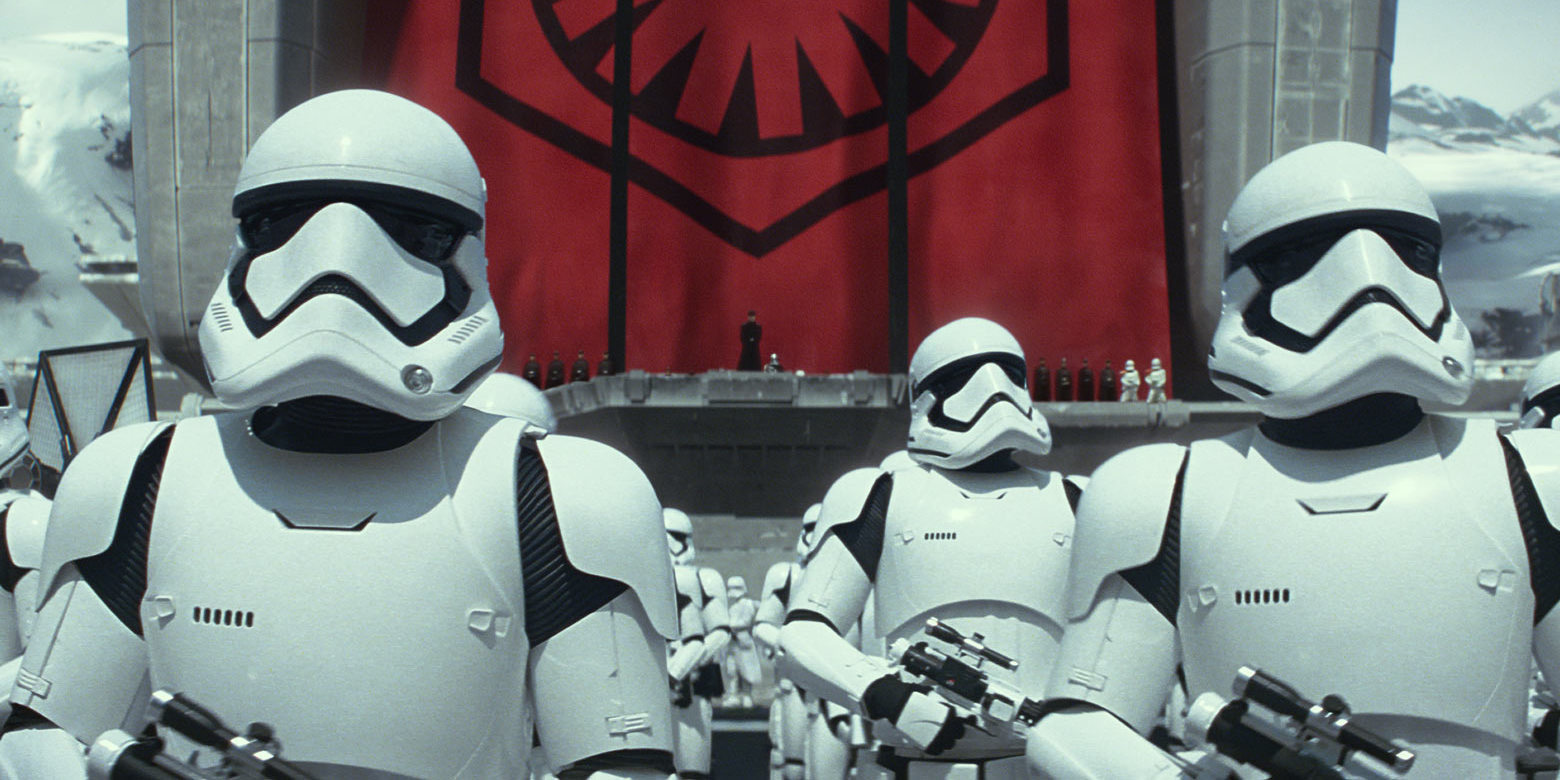
\includegraphics[width = 1\textwidth]{tla-introduction/first-order}
  \end{center}
\end{frame}

\begin{frame}
  \frametitle{First Order Logic}
  $Coaches \triangleq \{"A", "B"\}$

  $SeatNumbers \triangleq \{1, 2, 3, 4, 5, 6, 7, 8, 9, 10\}$

  $Seats \triangleq Coaches \times SeatNumbers$
\end{frame}

\begin{frame}
  \frametitle{First Order Logic}
  $Coaches \triangleq \{"A", "B"\}$

  $SeatNumbers \triangleq \{1, 2, 3, 4, 5, 6, 7, 8, 9, 10\}$

  $Seats \triangleq \{\langle"A", 1\rangle, \langle"B", 1\rangle,$
  
  $\langle"A", 2\rangle, \langle"B", 2\rangle,\langle"A", 3\rangle, \langle"B", 3\rangle,$
  
  $\langle"A", 4\rangle, \langle"B", 4\rangle,\langle"A", 5\rangle, \langle"B", 5\rangle,$
  
  $\langle"A", 6\rangle, \langle"B", 6\rangle,\langle"A", 7\rangle, \langle"B", 7\rangle,$
  
  $\langle"A", 8\rangle, \langle"B", 8\rangle,\langle"A", 9\rangle, \langle"B", 9\rangle,$
  
  $\langle"A", 10\rangle, \langle"B", 10\rangle \}$
\end{frame}

\begin{frame}
  \frametitle{First Order... Logic}
  $Predicate \triangleq i \in \{1, 2, 3, 4\}$
\end{frame}

\begin{frame}
  \frametitle{First Order Logic}

  $Implies \triangleq i \in \{1, 2\} \Rightarrow i \in \{1, 2, 3\}$
\end{frame}

\begin{frame}
  \frametitle{First Order Logic}
  $ConjuctionOp(seat) \triangleq seat[1] \in \{"A", "B"\} \land seat[2] \in 1..10$
\end{frame}

\begin{frame}
  \frametitle{First Order Logic}

  $Existence \triangleq \exists\ seat \in Seats : seat = \langle"A", 1\rangle$
  
  \begin{center}
    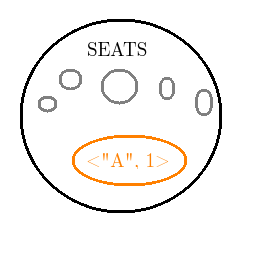
\includegraphics[width=0.5\textwidth]{tla-introduction/exists}
  \end{center}
\end{frame}

\begin{frame}
  \frametitle{First Order Logic}

  $Universal \triangleq \forall\ seat \in Seats : ConjuctionOp(seat)$
  
  \begin{center}
    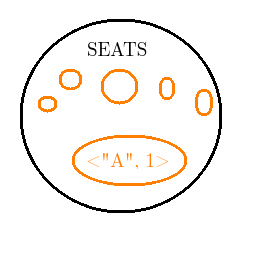
\includegraphics[width=0.5\textwidth]{tla-introduction/universal}
  \end{center}
\end{frame}

\begin{frame}
  \centering \Huge \emph{First Specification}
\end{frame}

\begin{frame}
  \frametitle{First Specification}
  
  $Union \triangleq \{1, 2\} \cup \{3\} = \{1, 2, 3\}$
\end{frame}

\begin{frame}
  \frametitle{First Specification}
  
  \begin{center}
    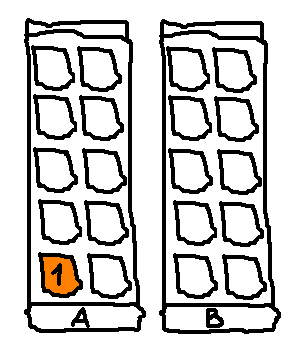
\includegraphics[width=0.5\textwidth]{tla-introduction/single-seat}
  \end{center}
\end{frame}

\begin{frame}
  \frametitle{First Specification}
  
  \begin{center}
    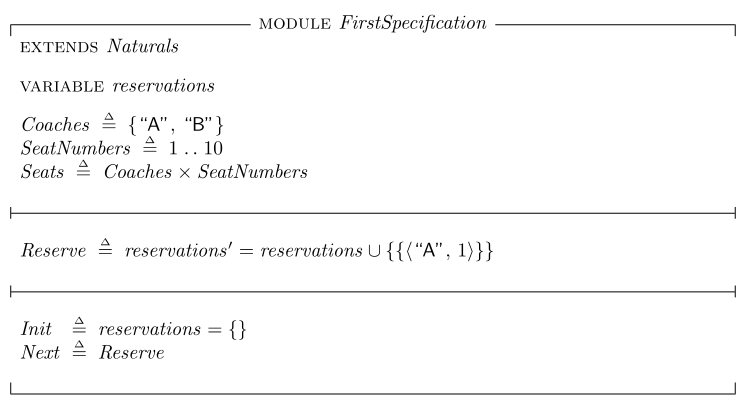
\includegraphics[width=0.9\textwidth]{tla-introduction/first-specification}
  \end{center}
\end{frame}

\begin{frame}
  \frametitle{First Specification}
  
  $\textsc{VARIABLE}\ reservations$
\end{frame}

\begin{frame}
  \frametitle{First Specification}

  $Reserve \triangleq reservations' = reservations \cup \{\langle"A", 1\rangle\}$
\end{frame}

\begin{frame}
  \frametitle{First Specification}
  
  $Init \triangleq reservations = \{\}$
  
  $Next \triangleq Reserve$
\end{frame}

\begin{frame}
  \centering \Large \emph{Toolbox}
\end{frame}

\begin{frame}
  \frametitle{Reserving a seat at a time}

  $Reserve \triangleq \exists\ seat \in Seats : reservations' = reservations \cup \{\{seat\}\}$
\end{frame}

\begin{frame}
  \centering \Huge \emph{Toolbox}
\end{frame}

\begin{frame}
  \frametitle{Enforcing an invariant}

  At most 70\% of the train is reserved
\end{frame}

\begin{frame}
  \frametitle{Enforcing an invariant}

  $Union \triangleq \textsc{UNION}\ \{\{1, 2, 3\}, \{1, 4\}\} = \{1, 2, 3, 4\}$
\end{frame}

\begin{frame}
  \frametitle{Enforcing an invariant}

  $Cardinal \triangleq Cardinality(\{1, 2, 3\}) = 3$
\end{frame}

\begin{frame}
  \frametitle{Enforcing an invariant}

  $70PercentTrainOccupation \triangleq (70 * Cardinality(Seats)) \div 100$
  
  $AtMost70PercentTrainOccupation \triangleq Cardinality(\textsc{UNION}\ reservations) \le 70PercentTrainOccupation$
\end{frame}

\begin{frame}
  \centering \Huge \emph{Toolbox}
\end{frame}

\begin{frame}
  \frametitle{Counter Example}
  
  \begin{center}
    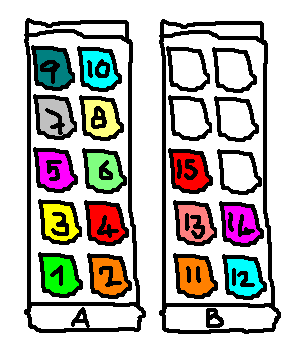
\includegraphics[width=0.5\textwidth]{tla-introduction/over-70-train-single-seat}
  \end{center}
\end{frame}

\begin{frame}
  \frametitle{Inforcing the invariant}
  
  $70PercentTrainOccupation \triangleq (70 * Cardinality(Seats)) \div 100$
  
  $ReservedSeats \triangleq \textsc{UNION}\ reservations$
  
  $Reserve \triangleq$
  
  $\land Cardinality(ReservedSeats) < 70PercentTrainOccupation$
  
  $\land \exists\ seat \in Seats : reservation' = reservations \cup \{\{seat\}\}$
\end{frame}

\begin{frame}
  \centering \Huge \emph{Reserving multiple seats}
\end{frame}

\begin{frame}
  \frametitle{Reserving multiple seats}
  
  $Subset \triangleq \textsc{SUBSET}\ \{1, 2, 3\} = \{\{\}, \{1\}, \{2\}, \{3\}, \{1, 2\}, \{2, 3\}, \{1, 3\}, \{1, 2, 3\}\}$
\end{frame}

\begin{frame}
  \frametitle{Reserving multiple seats}
  
  $Reserve(count) \triangleq$
  
  $\land Cardinality(ReservedSeats) < 70PercentTrainOccupation$
  
  $\land \exists\ seats \in \textsc{SUBSET}\ Seats :$
  
  $\land Cardinality(seats) = count$
  
  $\land reservation' = reservations \cup \{seats\}$
\end{frame}

\begin{frame}
  \frametitle{Reserving multiple seats}
  
  $Next \triangleq \exists\ seatCount \in 1..Cardinality(Seats) : Reserve(seatCount)$
\end{frame}

\begin{frame}
  \centering \Huge \emph{Toolbox}
\end{frame}

\begin{frame}
  \frametitle{Counter Example}
  
  \begin{center}
    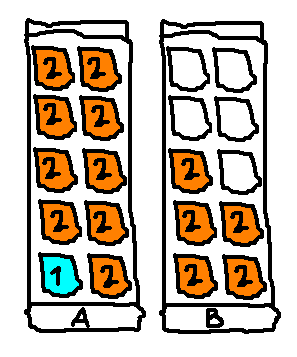
\includegraphics[width=0.5\textwidth]{tla-introduction/over-70-multiple-reservation}
  \end{center}
\end{frame}

\begin{frame}
  \frametitle{Reserving multiple seats}
  
  $Reserve(count) \triangleq$
  
  $\land Cardinality(ReservedSeats) < 70PercentTrainOccupation$
  
  $...$
\end{frame}

\begin{frame}
  \frametitle{Fixing the specification}
  
  $Reserve(count) \triangleq$
  
  $\land Cardinality(ReservedSeats) + count \le 70PercentTrainOccupation$
  
  $\land \exists\ seats \in \textsc{SUBSET}\ Seats :$
  
  $\land Cardinality(seats) = count$
  
  $\land reservation' = reservations \cup \{seats\}$
\end{frame}

\begin{frame}
  \centering \Huge \emph{Overlapping reservations}
\end{frame}

\begin{frame}
  \frametitle{Overlapping reservations}
  
  $SeatsReservedOnce \triangleq$
  
  $\forall\ seat \in Seats : \forall\ r1 \in reservations : \forall\ r2 \in reservations :$
  
  $(seat \in r1 \land seat \in r2) \Rightarrow r1 = r2$
\end{frame}

\begin{frame}
  \centering \Huge \emph{Toolbox}
\end{frame}

\begin{frame}
  \frametitle{Counter Example}
  
  \begin{center}
    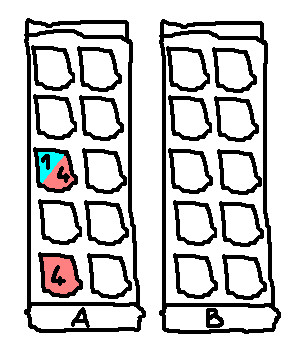
\includegraphics[width=0.5\textwidth]{tla-introduction/conflict-reservation}
  \end{center}
\end{frame}

\begin{frame}
  \frametitle{Overlapping reservations}
  
  $SetDifference \triangleq \{1, 2, 3\} \backslash \{3, 4\} = \{1, 2\}$
\end{frame}

\begin{frame}
  \centering \Huge \emph{Toolbox}
\end{frame}

\begin{frame}
  \frametitle{First Order Logic (FOL)}
  
  \begin{itemize}
  	\item Intuitive
  	\item Powerful
  	\item Most problems can be expressed with FOL
  \end{itemize}
\end{frame}

\begin{frame}
  \frametitle{TLA+}
  
  \begin{itemize}
  	\item Yields the power of FOL
  	\item Easy incremental modelling
  	\item Built for distributed systems
  \end{itemize}
\end{frame}

\begin{frame}
  \frametitle{Single node reservation}
  
  \begin{center}
    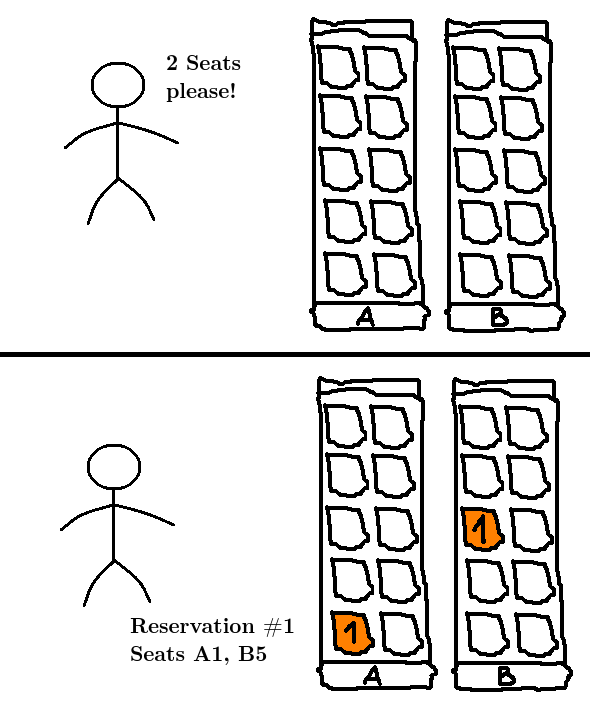
\includegraphics[width=0.5\textwidth]{tla-introduction/client-reserving}
  \end{center}
\end{frame}

\begin{frame}
  \frametitle{Distributed reservation}
  
  \begin{center}
    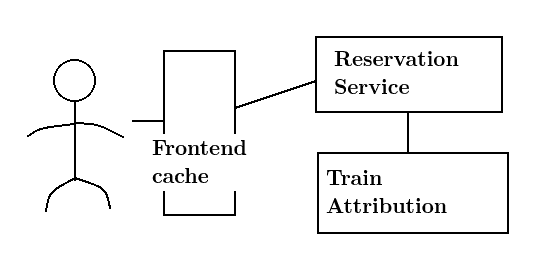
\includegraphics[width=0.5\textwidth]{tla-introduction/complex-system}
  \end{center}
\end{frame}

\begin{frame}
  \frametitle{What's next?}

  \begin{itemize}
  	\item Download the toolbox
  	\item Play with some tutorials
  	\item \href{https://groups.google.com/g/tlaplus}{Ask your questions to the community}
  	\item \href{https://www.informit.com/store/specifying-systems-the-tla-plus-language-and-tools-9780321143068}{Read the book}
  	\item Have fun!
  \end{itemize}
\end{frame}

\begin{frame}
  \centering \Huge \emph{Thank you}
\end{frame}

\end{document}
